\documentclass[12pt]{article}
\usepackage[utf8]{inputenc}
\usepackage[T5]{fontenc}
\usepackage{graphicx,a4wide,framed}

\newcommand{\source}[1]{\begin{flushright}\emph{[#1]}\end{flushright}}

\newcommand{\MakeScribeTop}[1]{
\noindent
\begin{framed}
\noindent
 Algorithmique Avancée 2018
 \hfill
 École Centrale-Supélec
 \\[1em]
 \centerline{ \Large
#1
 }
 \\[1em]
\centerline{  \it Christoph Dürr, Nguyễn Kim Thắng}
\end{framed}
}



\begin{document}
    \MakeScribeTop{Corrections}

    \section{Diviser pour régner et algorithme glouton}

    \subsection{Cartes bancaires}

    L'instance est graphe $G$ qui est une union disjointe de cliques. Les sommets sont numérotés de 1 à $n$. La seule manière d'accéder au graphe est de demander s'il existe une arête entre deux sommets $u,v$ donnés.  Le but est de décider s'il existe une clique de taille $\lceil n/2 \rceil$ au moins ou pas. Appelons une telle clique \emph{grande}.  Dans le cas positif, nous voulons également retourner cette clique, et non seulement annoncer son existence.

    On propose une solution par la méthode diviser et régner.
    Le cas de base~:
    Si le graphe contient moins de 2 sommets, la réponse est non. Si le graphe contient deux sommets la réponse est oui si ces sommets sont reliés par une arête.

    Pour des valeurs de $n$ supérieur à 2, on procède comme suit. D'abord on divise arbitrairement les sommets en deux parties disjointes $A,B$, avec $|A|=\lfloor n/2 \rfloor, |B|=\lceil n/2 \rceil$ (ou l'inverse).  Ensuite on considère le graphe $G_A$ induit par $A$, c'est à dire composé des sommets $A$ et des arêtes de $G$ ayant les deux extrémités dans $A$.  De même manière on considère le graphe $G_B$ induit par $B$.  Cette construction n'est faite que conceptuellement. À ce niveau là, l'algorithme ne fait que diviser les sommets en temps $O(n)$.

    L'observation clé est la suivante. Supponsons que le graphe $G$ contient une grande clique $S$. Alors au moins un des graphes $G_A, G_B$ contient également une grande clique.  Et chacune des grandes cliques de $G_A$ ou de $G_B$ fait partie de la grande clique $S$.

    On commence par rechercher récursivement une grande clique dans $G_A$ puis dans $G_B$.  Si les recherches n'ont rien donné, par l'observation clé, on peut répondre que $G$ n'a pas de grande clique.  Dans le cas contraire, les recherches ont revelé une grande clique dans un des graphes, disons une grande clique $S$ dans $G_A$.  On doit désormais tester si $S$ fait partie d'une grande clique dans $G$.  Pour cela on doit déterminer la plus grande clique dans $G$ contenant $S$.  On sait que les sommets de $A\setminus S$ ne sont pas reliés à $S$. Désormais on doit faire ce test pour tous les sommets de $B$.  Donc pour chaque sommet $v\in B$ on teste s'il est relié à $S$.  Comme $G$ est une collection de cliques, $v$ est soit disjoint de $S$ soit relié à tous les sommets de $S$. Il suffit donc de faire le test sur le couple de sommets $(u,v)$ où 
     $u$ est un sommet arbitraire dans $S$. 
     Si la clique $S'\supseteq S$ ainsi obtenue est grande pour $G$ on peut retourner cette clique, sinon par l'observation clé, on peut répondre que $G$ n'a pas de grande clique.

     \centerline{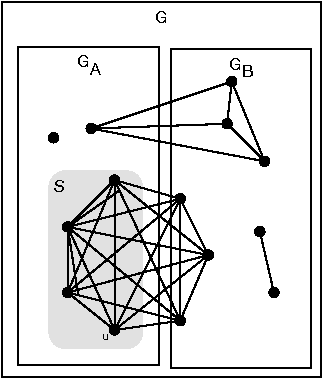
\includegraphics{grande_clique.pdf}}

     Pour l'analyse de la complexité, on note $T(n)$ une majoration sur le temps passé par l'algorithme pour un graphe de taille $n$.  On a $T(1) = T(2) = c$ pour une constante $c$, ainsi que $T(n) \leq 2\cdot T(\lceil n/2 \rceil)  + cn$ pour la même constante $c$ choisie suffisament grande.  En déroulant la récursion sur $T$ on obtient $T(n) \leq c n + c n  \lceil \log_2 n \rceil = O(n \log n)$.

    \subsection{Placement d'antennes}


\paragraph{Observation}
Quand on trace un cercle autour de chaque île de rayon $r$, on découvre un intervalle sur la plage qui doit contenir une antenne. Le problème se réduit alors au problème suivant.

\paragraph{Ensemble minimum de points intersectant chacun des intervalles donnés}
Pour $n$ intervalles donnés, il faut trouver un ensemble de points $S$ de cardinalité minimale tel que chaque intervalle intersecte $S$.

\paragraph{Algorithme glouton par balayage en $O(n\log n)$.}
On traite tous les intervalles dans l'ordre croissant de leur côté droit.  Ce tri coûte un temps $O(n \log n)$ est constitue le goulot d'étranglement. La suite ne prend qu'un temps linéaire.

À tout moment on maintient une solution $S$ pour les intervalles déjà vus, qui minimise $|S|$ et en cas d'égalité maximise $\max S$.

L'algorithme est simple.  Si pour un intervalle $[l,r]$ on a $l\leq max S$, alors on ne fait rien, sinon on ajoute $r$ à $S$.
L'idée est qu'il faut de toute façon couvrir $[l,r]$ et en choisissant la valeur la plus grande qui le couvre, on augmente la chance de couvrir également les intervalles traités par la suite.

Pour se convaincre de l'optimalité, soit $S$ une solution optimale pour l'ensemble $I$ des intervalles déjà vues ainsi que $[l,r]$.  Soit $S$ est déjà une solution pour $I$, et dans ce cas $l\leq \max S$, soit $S\backslash \max S$ est une solution optimale pour $I$.


\section{Programmation dynamique 1}

\subsection{Arbre binaire de recherche optimal}

Soit $A[i,j]$ le coût de l'arbre de recherche optimal pour le problème restreint aux éléments de $i$ à $j$.
 Notons $T[i,j]$ cet arbre.

  Les cas de base sont $A[i,i]=f_i$ et $A[i,i-1]=0$ pour l'arbre vide (Le cas $i=j$ n'est pas vraiement nécessaire d'être mentionné dans les cas de base). 
Pour $i<j$, l'arbre optimal a bien une racine, disons avec l'élément $k$ pour $i\leq k\leq j$.  

Observation clé: Le sous-arbre gauche est un arbre optimal pour les élements de $i$ à $k-1$, car si on pouvait le remplacer par un arbre meilleur ceci diminuerait également le coût de $T[i,j]$ et contredirait son optimalité.  Il en est de même pour le sous-arbre droit.

Donc $T[i,j]$ a la forme $\textrm{tree}(T[i,k-1],k,T[k+1,j])$ pour un certain $k$, et où tree dénote le constructeur d'un arbre binaire. Quel est le coût de l'arbre~?
Les éléments du sous-arbre gauche ont une profondeur plus grande dans $T[i,j]$ que dans $T[i,k-1]$. Il faut donc ajouter $f_i + \ldots f_{k-1}$ au coût de $T[i,k-1]$, qui par définition est $A[i,k-1]$.  On a la même situation avec sous-arbre droit. Et la racine génère un coût de $f_k$.  Ces observation mènent vers la récursion pour $i \leq j$
\[
	A[i,j] = f_i + \ldots + f_j +  \min_{i\leq k\leq j} (A[i,k-1] + A[k+1,j]).
\]


     \centerline{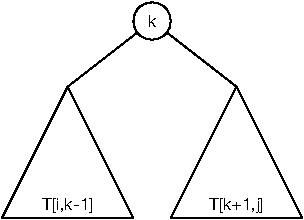
\includegraphics{abre_bin_rech_opt.pdf}}


On a $O(n^2)$ variables à calculer, chacune est une minimisation sur $O(n)$ alternatives. Au total la complexité est de $O(n^3)$.
Ces variables doivent être calculées dans un bon ordre. Une possibilité est de boucler sur toutes les valeurs $j=1,2,\ldots, n$ et à l'intérieur de boucler sur toutes les valeurs $i=j,j-1, j-2, \ldots, 1$ dans cet ordre.

Pour calculer l'arbre proprement dit il suffit de stocker dans une matrice auxiliaire $K$, la valeur $K[i,j]=k$ où $k$ est le minimiseur de la récursion pour $A[i,j]$.  Ensuite la fonction récursive \textsl{build\_tree}$(i,j)$ va retourner l'arbre vide si $j<i$ et sinon retournera 
\[
\textrm{tree}(\textsl{build\_tree}(i,K[i,j]-1), K[i,j], \textsl{build\_tree}(K[i,j]+1,n)).
\]
Cette construction aura une complexité linéaire en $n$ car un travail constant est effectué pour chaque nœud.


\subsection{Distance d'édition}

Similaire à la plus longue sous-séquence commune.
Sous-problème défini par les préfixes $x_1,\ldots,x_i$ et $y_1,\ldots,y_j$.
Soit $A[i,j]$ la distance d'édition entre ces préfixes. 
Cas de base: $A[0,j]=j$ insertions et $A[i,0]=i$ suppressions.
Si $x_i=y_j$, alors il existe une solution optimale qui ne touche pas à ces deux lettres et $A[i,j]= A[i-1,j-1]$ dans ce cas.

Sinon, si $x_i\neq y_j$ forcément au moins une des lettres a subi une des trois opérations, et donc dans ce cas
\[
A[i,j] = 1 + \min\{ \underbrace{A[ i,j-1 ]}_{\textrm{insertion $y_j$}}, 
 \underbrace{A[i-1,j]}_{\textrm{suppression $x_i$}}, 
 \underbrace{A[i-1,j-1]}_{\textrm{substitution $x_i \rightarrow y_j$}} \}.
\]

\subsection{Partage équitable}

Notons $W=\sum w_i$.  Pour $0\leq v \leq W$ et $0 \leq i \leq n$, soit $T[i,v]$ un booléen qui indique s'il existe un ensemble $S\subseteq \{1, \ldots, i\}$ avec $\sum_{j\in S} w_j = v$.

Les cas de base sont $T[0,0]=$Vrai et $T[0,v]=$Faux pour tout $v>0$.
Sinon pour $i \leq 1$ et $v$ fixé l'ensemble de somme $v$ soit contient $i$ soit ne contient pas $i$.  Ceci donne la récursion suivante
\[
		T[i,v] = T[i-1, v] \vee T[i-1, v - w_i],
\]
où la dernière option n'est valable que si $v \geq w_i$.

Enfin le partage équitable peut être obtenu en cherchant la valeur $v$ la plus proche de $\sum w_i /2$ pour laquelle on ait $T[n,v]$.  Pour obtenir l'ensemble proprement dit, il faut maintenir dans un tableau auxiliaire lequel des deux choix de la récursion ci-dessous a rendu $T[i,v]$ vrai. Ceci permet de dérouler dans l'ordre décroissant des indices $i$, les éléments de l'ensemble $S$ de la solution.

\end{document}